\documentclass{article}

\usepackage{amsmath, amsfonts, amssymb, amsthm}
\usepackage{tikz}

\theoremstyle{plain}
\newtheorem{theorem}{Theorem}[section]
\newtheorem{proposition}[theorem]{Proposition}

\title{Every square can be tiled with T-tetrominos and no more than 5 monominos}
\author{Jack Grahl}

\begin{document}
\maketitle

\begin{abstract}
If $n$ is a multiple of 4, then a square of side $n$ can be tiled with T-tetrominos, using a well-known construction.
If $n$ is even but not a multiple of four, then there exists an equally well-known construction for tiling a square of side $n$ with T-tetrominos and exactly 4 monominos.
On the other hand, it was shown by Walkup in \cite{walkup} that it is not possible to tile the square using only T-tetrominos.
Now consider the remaining cases, where $n$ is odd.
It was shown by Zhan in \cite{zhan} that it is not possible to tile such a square using only one monomino.
Hochberg showed in \cite{hochberg} that no more than 9 monominos are ever needed.
We give a construction for all odd $n$ which uses exactly 5 monominos, thereby resolving this question.
Hochberg also conjectured that no more than 5 monominos are needed for any rectangle.
Our construction can also be used for some classes of rectangles with odd width and height, other than squares, and reduces the space of possible counter-examples.
\end{abstract}

\begin{theorem}
Every square can be tiled with T-tetrominos and at most 5 monominos.
\end{theorem}
This theorem follows immediately from propositions \ref{four}, \ref{even} and \ref{odd}.

\begin{proposition}\label{four}
Every square of side $n = 4m$ can be tiled with T-tetrominos.
\end{proposition}
This was stated by Walkup in \cite{walkup}, who simply pointed out that it is an obvious consequence of the fact that the square of side 4 can be tiled, which is itself easy to check.

\begin{proposition}\label{even}
Every square of side $n = 4m + 2$ can be tiled with T-tetrominos and 4 monominos, and 4 monominos are always needed.
\end{proposition}
For $n = 2$ this is the same as pointing out that a single T-tetromino will not fit in the $2x2$ square.
For $n=6$ and above, Walkup's Theorem 1 (\cite{walkup}) shows that it is not possible to tile the square without monominos.
Clearly at least 4 are needed.
As Hochberg points out in Theorem 8 of \cite{hochberg}, a tiling with only tetrominos of a rectangle whose sides are both multiples of 4, can be extended to a tiling of a rectangle which is bigger by 2 in each direction, using only 4 monominos.
The L-shaped strip which is added to the former looks (for example) like Figure \ref{lshaped}.

\begin{figure}\label{lshaped}
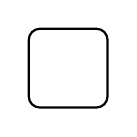
\begin{tikzpicture}
\draw [rounded corners, thick] (0,0.5) -- (0,1) -- (1,1) -- (1,0) -- (0,0) -- (0,0.5);
\end{tikzpicture}
\caption{The L-shaped strip which extends any square of side $4n$ to a square of side $4n+2$, using exactly 4 monominos.}
\end{figure}

\bibliography{polyomino}{}
\bibliographystyle{plain}
\end{document}
